\documentclass[border=0.2cm]{standalone}
\usepackage{tikz}
\usetikzlibrary{calc, angles, quotes}
\usetikzlibrary{intersections} % Necessário para achar pontos de cruzamento

\begin{document}
\pagestyle{empty}

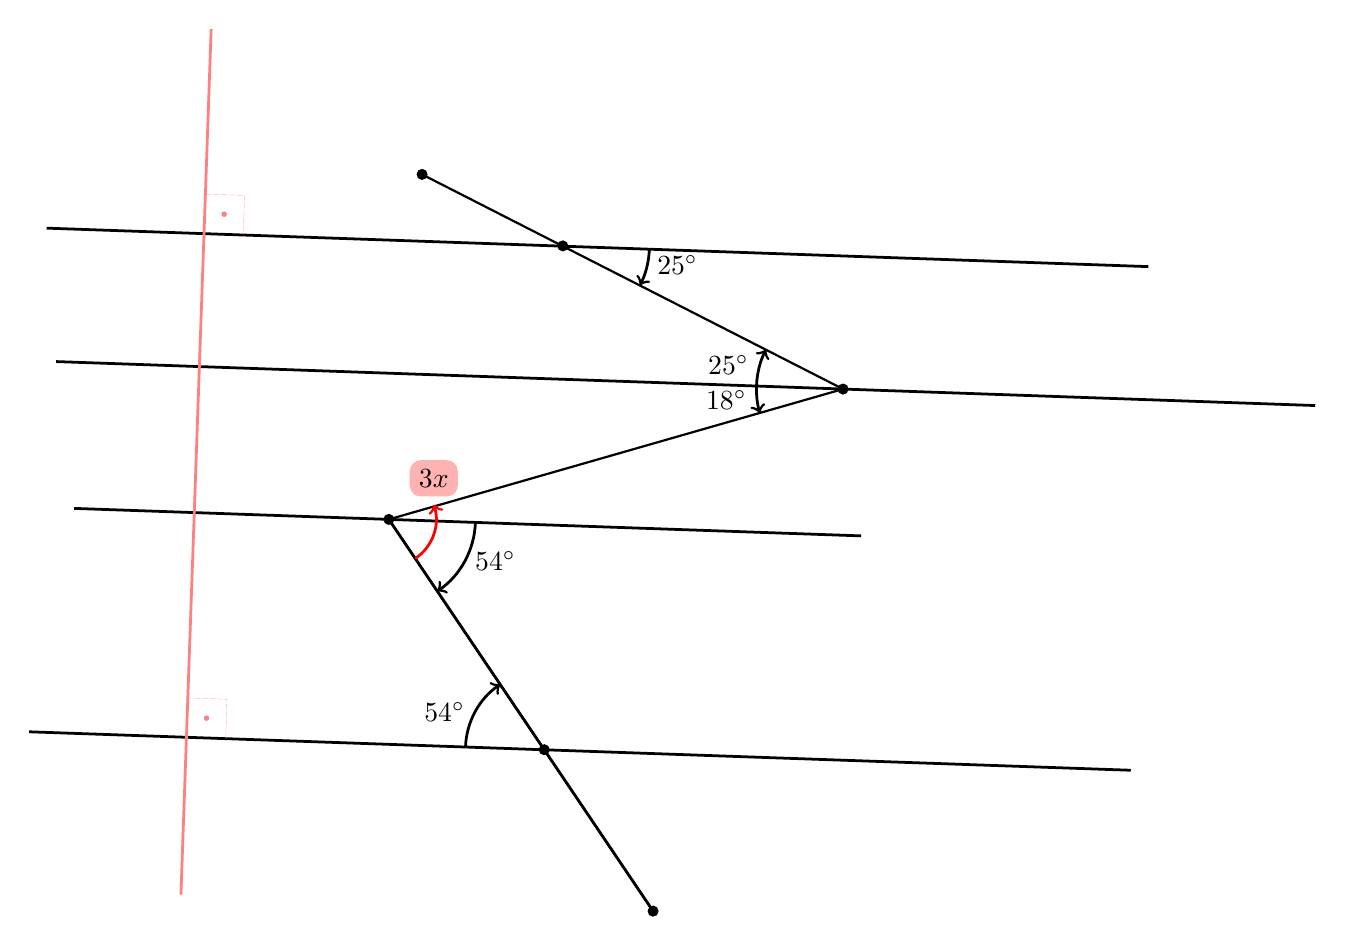
\begin{tikzpicture}[scale=2,line width=1pt,rotate=-2]
           
    \coordinate (A) at (0,0);
    \coordinate (B) at (180-54:3cm);
    \coordinate (C) at ($(B)+(18:3cm)$);
    \coordinate (D) at ($(C)+(180-25:3cm)$);
    
    \draw[thick] (A) -- (B) -- (C) -- (D);
    

    \draw (B) -- +(3,0) -- +(-2,0);
    \draw (C) -- +(3,0) -- +(-5,0);

    \draw[name path=lineD] (-4,4.2) -- +(7,0);
    \draw[name path=lineA] (-4,1) -- +(7,0);

    \fill (A) circle (1pt); % node[above left] {A};
    \fill (B) circle (1pt); % node[above left] {B};
    \fill (C) circle (1pt); % node[above left] {C};
    \fill (D) circle (1pt); % node[above left] {D};

    \draw[name path=AB] (A) -- (B);
    \path[name path=CD] (C) -- (D);
     
    \draw[name path=lineR,red!50] (-3,0) -- (-3,5.5); 


    \path[name intersections={of=lineD and CD}] coordinate (interA)  at (intersection-1);
    \path[name intersections={of=lineA and AB}] coordinate (interB)  at (intersection-1);
    \path[name intersections={of=lineR and lineA}] coordinate (interC)  at (intersection-1);
    \path[name intersections={of=lineR and lineD}] coordinate (interD)  at (intersection-1);


    \fill (interA) circle (1pt); % node[above right] {interA};
    \fill (interB) circle (1pt); % node[above right] {interB};
   
    \coordinate (interCy) at ($(interC)+(.3,0)$);
    \coordinate (interCx) at ($(interC)+(0,.3)$);
    \coordinate (interCp) at ($(interC)+(.25/2,.25/2)$);
    \coordinate (interDy) at ($(interD)+(.3,0)$);
    \coordinate (interDx) at ($(interD)+(0,.3)$);
    \coordinate (interDp) at ($(interD)+(.25/2,.25/2)$);
    
    %\coordinate (interC2) at (0,0);

    \draw[red!50] (interC) pic [line width=.05pt, draw, angle eccentricity=1.5, angle radius=5mm] {right angle=interCx--interC--interCy};
    \fill[red!50] (interCp) circle (.5pt);
    \draw[red!50] (interD) pic [line width=.05pt, draw, angle eccentricity=1.5, angle radius=5mm] {right angle=interDx--interD--interDy};
    \fill[red!50] (interDp) circle (.5pt); 
    
% Arco 1 vermelho (B) (interB)
    \draw[<-] ($(interB)+(180-54:5mm)$)  arc (180-54:180:5mm) node[midway,left] {$54^\circ$};
    \draw[->] ($(B)+(0:5.5mm)$)  arc (0:-54:5.5mm) node[midway,right] {$54^\circ$};
    %\draw[black!50,->] ($(interB)+(0:7mm)$)  arc (0:360:7mm);

% Arco 2 azul (B) (C)
   \draw[red,->] ($(B)+(-54:3mm)$)  arc (-54:20:3mm) node[above,yshift=.5pt,fill=red!30,text=black,rounded corners,yshift=2pt] {$3x$};
   \draw[->] ($(C)+(180:5.5mm)$)  arc (180:180+18:5.5mm) node[midway,left] {$18^\circ$};

% Arco 2 azul (C) (interA)
   \draw[->] ($(C)+(180:5.5mm)$)  arc (180:180-25:5.5mm) node[midway,left,yshift=1pt] {$25^\circ$};
   \draw[->] ($(interA)+(0:5.5mm)$)  arc (0:-25:5.5mm) node[midway,right,yshift=1pt] {$25^\circ$};

\end{tikzpicture}

\end{document}